\chapter{GARCH}
\label{GARCH}
The Generalized Autoregressive Conditional Heteroskedasticity (GARCH) model is widely used in finance to analyse timeseries.

The model describes the variance of the current error term as a function of the previous error terms and the previous variances. The general formulationc can be written as:
\begin{equation}
    \sigma^2_t = a_{0} + \sum^{p}_{i=1}a_1 \epsilon^2_{t-i} + \sum^{q}_{j=1}a_2 \sigma^2_{t-j}
\end{equation}
Here $\sigma^2_t$ is the variance of the error term ad time $t$, $\epsilon^2_{t-i}$ is the squared error term at time $t-i$, $\sigma^2_{t-j}$ is the variance of the error term $j$ timesteps before $t$ and $a_0, a_1, a_2$ are the parameters of the model.

Considering the results obtained with the Autoregressive Model, we opted for an AR(1) for the mean of the timeseries and a GARCH(1,1) model for the variance of the error. The final model can be formalized in the following way:
\begin{equation}
    \begin{split}
        y_{t} = \mu_{0} + \epsilon_t + \alpha y_{t-1} \quad \epsilon_t \sim \mathcal{N}(0, \sigma^2_t) \\
        \sigma^2_t = a_{0} + a_1 \epsilon^2_{t-1} + a_2 \sigma^2_{t-1}
    \end{split}
\end{equation}

GARCH(1,1) + AR(1)
The likelihood of the GARCH model can be expressed as:
\begin{equation}
    y_{t}|\mu_{0},\alpha,y_{t-1},a_0,a_1,a_2,\sigma^2_{t-1}\sim \mathcal{N}(\mu_{0} + \alpha y_{t-1}, a_0 + a_1 \epsilon^2_{t-1} + a_2 \sigma^2_{t-1})
\end{equation}
We chose the following priors:
\begin{equation}
    \begin{split}
        \mu_0 \sim \mathcal{N}(0.0, 10000) \\
        \alpha \sim \mathcal{U}(-1.0, 1.0) \\
        a_0 \sim \mathcal{G}(0.01, 0.01) \\
        a_1 \sim \mathcal{G}(0.01, 0.01) \\
        a_2 \sim \mathcal{G}(0.01, 0.01)
    \end{split}
\end{equation}
We opted for an uninformative prior for $\mu_{0}$ and a uniform distribution for $\alpha$ to respect the stationary constraint for the AR part. Instead for $a_0, a_1, a_2$ we chose a gamma distribution in order to have a positive prior for the variance.
Here below are shown the posterior distributions for the parameters, while the traceplots and autocorrelation plots are provided in the Appendix.
\begin{figure}[h]
    \centering
    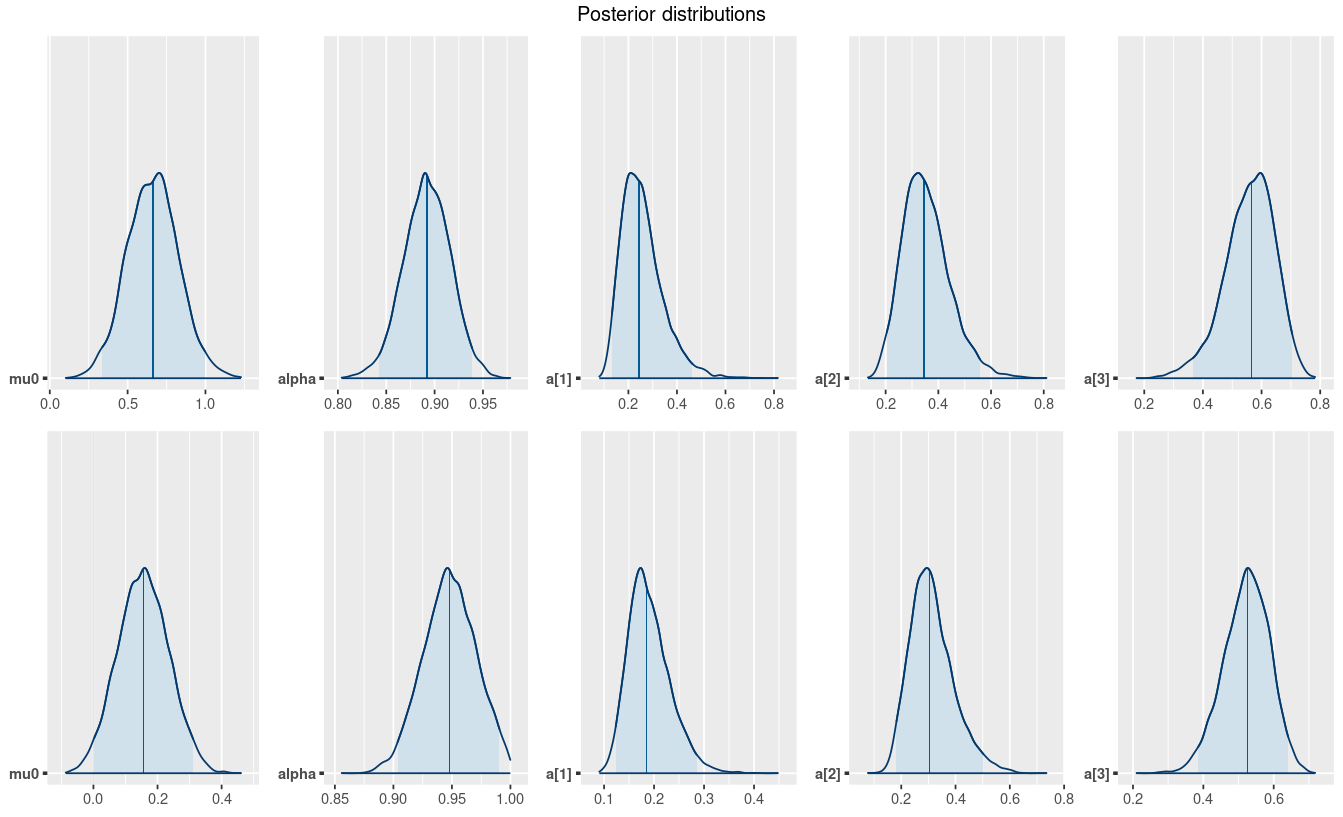
\includegraphics[width=\textwidth]{../Images/5-GARCH/posteriors.png}
    \caption{The image displays the posterior distributions of the parameters for the GARCH(1,1) model. The top line corresponds to the model used for GDP, while the bottom line corresponds to the model used for inflation.}
    \label{fig:GARCH_posteriors}
\end{figure}

Once we assested the validity of the results, we plotted the in-sample and out-of-sample prediction with credible intervals and we compared it with the true data:
\begin{figure}[h]
    \centering
    \begin{minipage}[t]{0.7\textwidth}
        \centering
        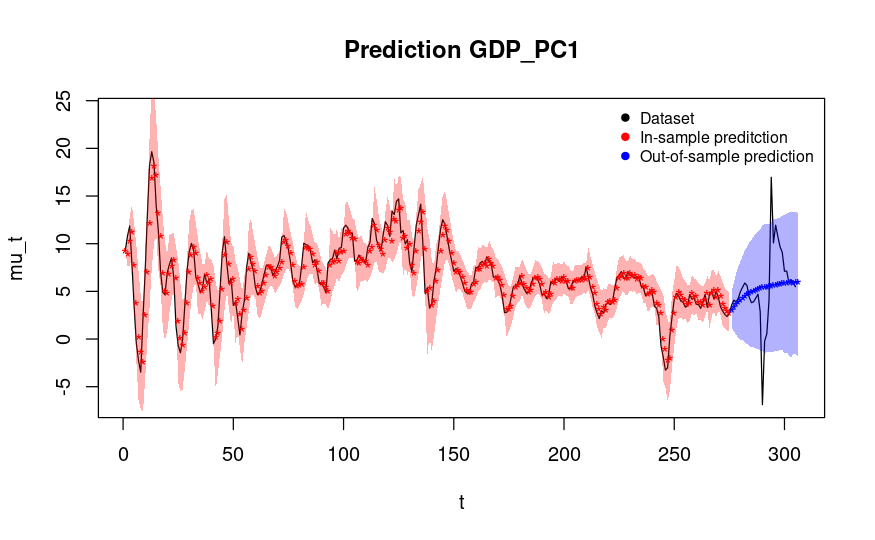
\includegraphics[width=\textwidth]{../Images/5-GARCH/gdp_prediction.png}
        \label{fig:GARCH_first}
    \end{minipage}
    \begin{minipage}[t]{0.7\textwidth}
        \centering
        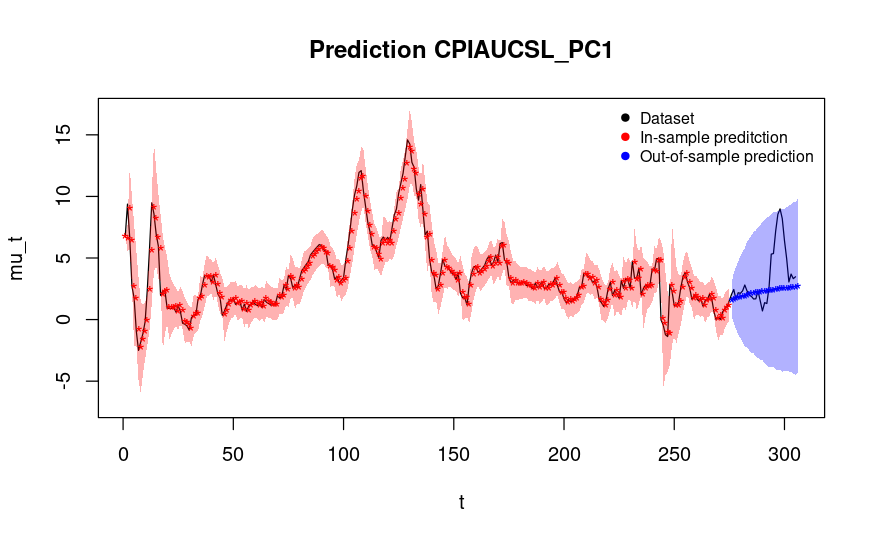
\includegraphics[width=\textwidth]{../Images/5-GARCH/infl_prediction.png}
        \label{fig:GARCH_second}
    \end{minipage}
    \caption{GARCH(1,1): In-sample and out-of-sample predictions}
    \label{fig:GARCH_combined}
\end{figure}
Finally we compared the model with the results from the uGarch library. The detailed comparison results are provided in the Appendix. 